\section{Context}
\label{sec:context}
\subsection{Self-nested trees and definitions}

In this report, we will only consider rooted unordered trees, % which
% set will be 
denoted by $\mathcal{T}$. Unordered trees are trees for
which the order among the children of a same node is not significant.
Let $v$ be a node of $T$, the complete subtree of $T$ rooted in $v$ will be
denoted by $T[v]$.

Two trees $T_{1} = (V_{1},E_{1})$ and  $T_{2} = (V_{2},E_{2})$ are
said to be isomorphic if there exists a bijection $f$ from  
$V_{1}$ to  $V_{2}$ such that for each pair of nodes $(u,v)$ in  $V_{1}$,
$(u,v) \in E_{1}$ if and only if $(f(u),f(v)) \in E_{2}$.

Let us consider the equivalence relation $\equiv$ on $\mathcal{T}$
defined by $T_1 \equiv T_2$ if and only if $T_1$ and $T_2$ are
isomorphic. More generally, we will say that two nodes $v_1$ and 
$v_2$ of $T$ , are equivalent if the subtrees
$T[v_1]$ and $T[v_2]$ are isomorphic. We will denote the
equivalence class of $v$ by $C(v)$.

A self-nested tree is a tree whose subtrees of identical height are
isomorphic to one another. An exemple of tree that is not self-nested
is given Figure \ref{fig:treeexample}, an example of self-nested tree is given
Figure \ref{fig:SNtree}.  We will denote $\mathcal{S}$
the set of the self-nested trees.

\begin{figure}[h]
 \begin{subfigure}[b]{0.45\textwidth}
    \centering  
    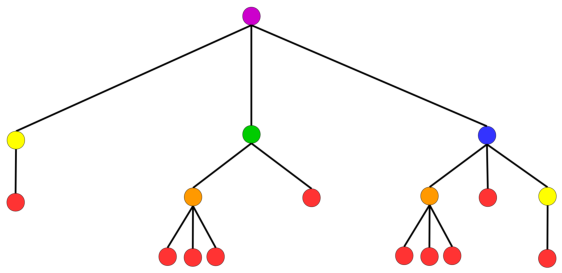
\includegraphics[width=\textwidth]{figures/tree2.pdf}
    \caption{Example of regular tree}
    \label{fig:treeexample}
  \end{subfigure}
  \quad
  \begin{subfigure}[b]{0.45\textwidth}
    \centering  
    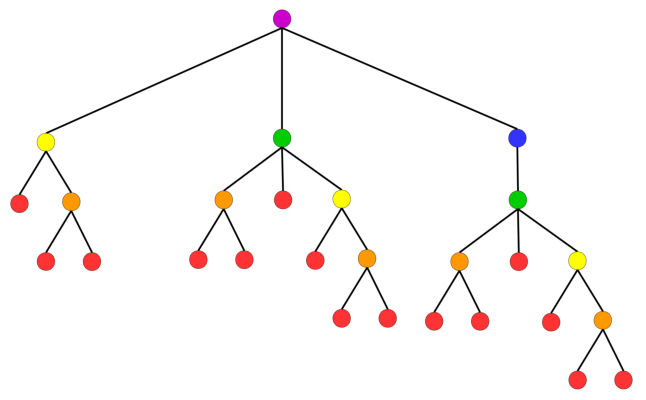
\includegraphics[width=\textwidth]{figures/tree.pdf}
    \caption{Example of self-nested tree}
    \label{fig:SNtree}
  \end{subfigure}
 
  \caption{Difference between regular trees and self nested trees}
\end{figure}

\subsection{DAG compression}

For $T = (V,E) \in \mathcal{T}$, let 
$\mathcal{Q}(T) = (V_{\mathcal{Q}}, T_{\mathcal{Q}})$ be the quotient
graph of $T$
by the equivalence relation $\equiv$. In concrete terms,
$V_{\mathcal{Q}} = \{ C(v) | v \in V \}$ is the quotient set of $V$ by
$\equiv$ and 
${E_{\mathcal{Q}} = \{ (C(u), C(v)) | (u,v) \in T \}}$.
Let $\delta$ be the weighting function on $\mathcal{Q}(T)$
defined by $$\delta(C(u), C(v)) = \#\{ v' \in Child(u) | C(v) = C(v')\}$$

The subfigure \ref{fig:dagexample} the quotient graph
corresponding to the tree represented Subfigure \ref{fig:treeexample}. The
equivalent nodes are represented in the same color.

\begin{figure}[h]
  \begin{subfigure}[b]{0.45\textwidth}
    \centering
    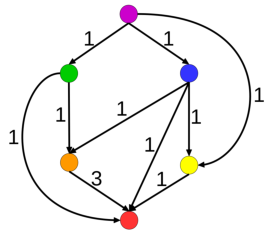
\includegraphics[width=.5\textwidth]{figures/dag2.pdf}
    \caption{DAG compression of the tree Subfigure \ref{fig:treeexample}}
    \label{fig:dagexample}
  \end{subfigure}
  \quad
  \begin{subfigure}[b]{0.45\textwidth}
    \centering
    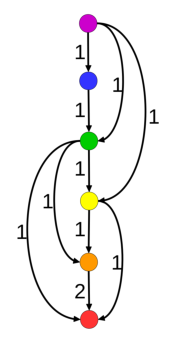
\includegraphics[width=.3\textwidth]{figures/dag.pdf}
    \caption{DAG compression of the tree Subfigure \ref{fig:SNtree}}
    \label{fig:SNdag}
  \end{subfigure} 
  \caption{Example of DAG compression}\label{fig:example}
\end{figure}

Let $T \in \mathcal{T}$, C. Godin and P. Ferraro showed in
\cite{godin} that $\mathcal{Q}(T)$ is a weighted directed acyclic
graph (\emph{DAG}) and that for each \emph{DAG} $Q$ with a weighting
function $\delta$, there exists a single tree $T \in \mathcal{T}$ such
as $\mathcal{Q}(T) = Q$.

The trees whose quotient graph is a linear \emph{DAG} (\emph{DAG} for
which there exists a hamiltonian path) are exactly the self-nested
trees. Since the nodes of equal height in a self-nested tree are
isomorphic to one anoter, there is a single vertex in the \emph{DAG}
for each height: the tree Subfigure \ref{fig:SNdag} is the quotient
graph of the self-nested tree represented Subfigure
\ref{fig:SNtree}. As a result, the number of vertices in the
\emph{DAG} is equal to the height of the initial tree.

\subsection{Avantages of self-nested trees}

Self-nested trees have a linear quotient graph, as a result they are
cheaper to store, but there are other advantages...

Let $T \in \mathcal{T}$ and $f$ be a recursive function ($f(u)$ depends
only on the values $(f(u_{i}))_{i \in I}$ where $(u_{i})_{i \in I}$
are the children of $u$). For example, $f$ can be the height or the
number of vertices of the subtree rooted in $u$. Since $f$ is
recursive, $f$ takes the same value on all the subtrees of $T$
isomorphic to one another, and computing $f$ on $T$ leads to make the
same computation several times. Thus, computing $f(T)$ directly on the DAG
corresponding to $T$ is more efficient than computing it on $T$ itself.

For example on Figure \ref{fig:compute} we can compute the number of
nodes directly on the DAG: the number of nodes under a leaf (red node)
is equal to one, the number of nodes under the orange nodes in $T$ is
equal to three times the number of nodes under a leaf plus one, that
is four. We can carry one the computation, at the end the number of
recursive calls will be equal to the number of nodes in the DAG
instead of the number of nodes in the tree (as it would have been if
we had computed $f$ on the tree).  Thus, the computation of recursive
functions is particularly efficient on self-nested trees because of the
small size of their DAG.

\begin{figure}[h]
  \centering
  \begin{subfigure}[b]{0.5\textwidth}
    \centering  
    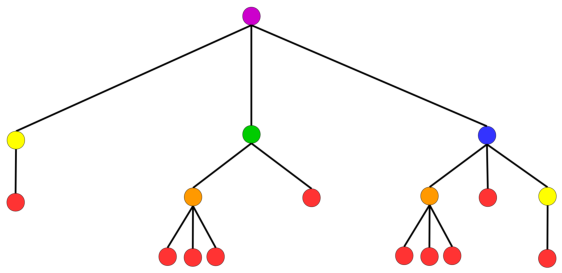
\includegraphics[width=\textwidth]{figures/tree2.pdf}
    \caption{Example of tree}
  \end{subfigure}
  \quad 
  \begin{subfigure}[b]{0.4\textwidth}
    \centering
    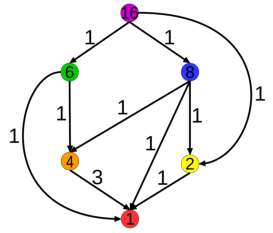
\includegraphics[width=.7\textwidth]{figures/dag2_nb_node.pdf}
    \caption{Computation of the number of nodes directly on its DAG}
    \label{fig:computeondag}
  \end{subfigure}
  \caption{Example of computation on the DAG}\label{fig:compute}
\end{figure}

Self-nested trees are a particularly relevant model of the structure
of a plant and are therefore usefull for the study of their
growth. Indeed, meristems are the tissues responsible for the growth
and some studies support the idea that the meristems of a plant go
through successive developement stages during their lives
\cite{meristems}. Furthermore, the transitions from one stage to
another occur in the same way for all the meristems of a same plant
and are specific to the species. We can indeed observe that the way
plants grow, the branching structure of their stems and branches seem
to follow some regular pattern repeated in several places in the
plant. Thus, representing the structure of the plant by a self-nested
tree whose nodes are the meristems and edges are the stems or branches
of the plant is natural and appropriate.

Unfortunately, a real plant has few chances to have exactly the
structure of a self-nested tree. Indeed, environmental conditions
(such as light and nutrition for example) also impact the growth of
the plant. This is one of the reasons why we are interested in
approximating trees by self-nested ones.

\subsection{Edit distance}
Let us consider the two following edit operations: the deletion and
addition of a node. Deleting a node $u$ in a tree means making the
children of $u$ children of the father of $u$ before removing $u$ from
the tree (Figure \ref{fig:deletion}). Adding a node is the
complementary operation, thus adding a node $u$ under $v$ means making
a subset of the children of $v$ become children of $u$ before placing
$u$ under $v$ (Figure \ref{fig:addition}).

\begin{figure}[h]
  \centering
  \begin{subfigure}[b]{0.3\textwidth}
    \centering  
    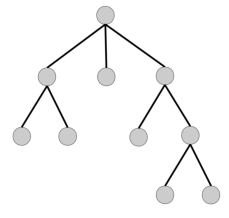
\includegraphics[width=.8\textwidth]{figures/edit.pdf}
    \caption{Initial tree}
  \end{subfigure}
  \begin{subfigure}[b]{0.3\textwidth}
    \centering
    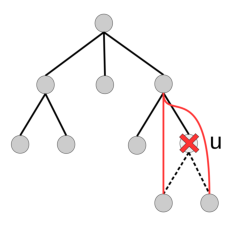
\includegraphics[width=.8\textwidth]{figures/edit_deletion.pdf}
    \caption{Deleting a node}
    \label{fig:deletion}
  \end{subfigure}
  \begin{subfigure}[b]{0.3\textwidth}
    \centering
    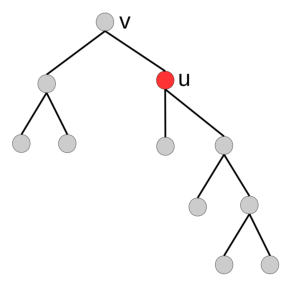
\includegraphics[width=\textwidth]{figures/edit_addition.pdf}
    \caption{Adding a node}
    \label{fig:addition}
  \end{subfigure}
  \caption{Example of edit operations}\label{fig:edit}
\end{figure}

Let $T_{1} = (V_{1},E_{1})$ and $T_{2} = (V_{2},E_{2})$ be two
trees. 

An edit sequence is a succession of edit operations. We can define the
cost of an edit sequence by the number of edit operations that were done.

An edit mapping between $T_{1}$ and $T_{2}$ is
a function $\Phi : V'_{1} \rightarrow V'_{2}$ where
$V'_{1} \subseteq V_{1}$ and $V'_{2} \subseteq V_{2}$, such as $\Phi$
is a bijection and preserves ancestrality among the nodes (in other
words, $u \in V'_{1}$ is an ancestor of  $v \in V'_{1}$ if and only if
$\Phi(u)$ is an ancestor of $\Phi(v)$). 

Given an edit mapping $\Phi$ between $T_{1}$ and $T_{2}$, there exists
a natural edit sequence leading from $T_{1}$ to $T_{2}$: every node
belonging to $V_{1} \setminus V'_{1}$ is deleted and every node in
$V_{2} \setminus V'{2}$ is added. Thus, we can define the cost of an
edit mapping $\Phi$ as the number of nodes that were added or deleted:
${\#(V_{1} \setminus V'_{1}) + \#(V_{2} \setminus V'_{2})}$.

More precisely, K.Zhang showed in \cite{zhang} that for every edit
mapping between $T_{1}$ and $T_{2}$ there exists a edit sequence of
equal cost. He also showed that for every edit sequence of $k$
operations leading from $T_{1}$ to $T_{2}$, there exists an edit
mapping of cost less than $k$.

It is also possible to define the edit distance between the trees
$T_{1}$ and $T_{2}$ as the minimal cost of an edit mapping between the
two trees (the properties of symmetry, identity of indescernibles and
triangle inequality are satisfied). We will notice that the minimal
cost of an edit mapping between $T_{1}$ and $T_{2}$ is also the
minimal cost of an edit sequence leading from $T_{1}$ to $T_{2}$
(result from the preceding properties shown in \cite{zhang}). 

In \cite{NPCzhang} K. Zhang, R. Statman and D. Shahsha show that the
problem of computing the edit distance between two trees is
NP-complete. There are several ways to overcome this difficulty: one
of them consists in restricting the set of instances to consider a set
of trees in which the distance is easier to compute. Another one consists
in modifying slightly the distance, for example by adding other
constraints, in order to build a new edit distance easier to compute.

The article \cite{zhang} presents an additional, sufficient and not
very constraining condition on the edit mapping along with a
polynomial algorithm to compute the new distance. The condition on the
edit mapping is the following: for all $u,v,w \in V'_{1}$, the least
common ancester of $u$ and $v$ is a proper ancester of $w$ if and only
if the least common ancestor of $\Phi(u)$ and $\Phi(v)$ is a proper
ancestor of $\Phi(w)$. In other words, $\Phi$ preserves the sibling
relation among the nodes: a node can be deleted only if all his
descendant are deleted as well or if all his siblings have been
deleted; during the addition of a new node $u$ under $v$, all the
children of $v$ have to become children of $v$ or none of them.

In this article, we will use this edit distance with its new
constraint.

\subsection{Approximation by self-nested trees}

As we explained before, a real plant has few chances to have an exact
self-nested structure. Therefore, approximating the trees of the
structure of different plants by self-nested trees could allow us to
find the theorical growth model of each species and thereby lead to a
better understanding of the evolution of the meristems.

If the goal is to compute the value taken by a recursive function $f$
on a tree $T$, approximating $T$ by a self-nested tree $S$ allows us to
compute very effectively $f(S)$, which can, under certain conditions,
be an approximative value of $f(T)$. 

\begin{figure*}
  \centering
  \begin{subfigure}[b]{0.475\textwidth}
    \centering
    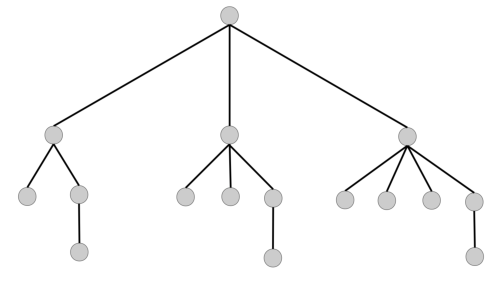
\includegraphics[width=\textwidth]{figures/T.pdf}
    \caption{$T$}    
    \label{fig:T}
  \end{subfigure}
  \hfill
  \begin{subfigure}[b]{0.475\textwidth}  
    \centering 
    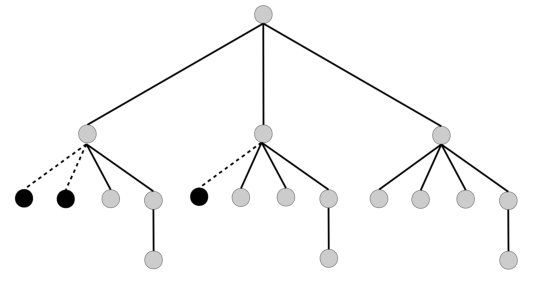
\includegraphics[width=\textwidth]{figures/NEST(T).pdf}
    \caption{$NEST(T)$}    
    \label{fig:NEST(T)}
  \end{subfigure}
  \vskip\baselineskip
  \begin{subfigure}[b]{0.475\textwidth}   
    \centering 
    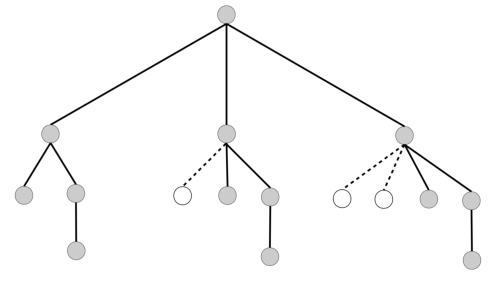
\includegraphics[width=\textwidth]{figures/NeST(T).pdf}
    \caption{$NeST(T)$}    
    \label{fig:NeST(T)}
  \end{subfigure}
  \quad
  \begin{subfigure}[b]{0.475\textwidth}   
    \centering 
    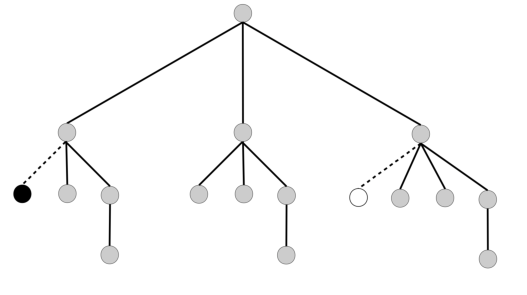
\includegraphics[width=\textwidth]{figures/NST(T).pdf}
    \caption{$NST(T)$}    
    \label{fig:NST(T)}
  \end{subfigure}
  \caption{Different approximations of $T$ by self-nested trees} 
  \label{fig:approx}
\end{figure*}
    
Several meanings can be given to the term ``approximating a tree by a
self-nested one''. For example, C. Godin and P. Ferraro have proposed a
polynomial algorithm \cite{godin} to compute the NEST (Nearest
Embedding Self-nested Tree) of a tree $T$. The NEST of $T$ is the
self-nested tree $S$ that minimize the edit distance between $S$ and
$T$ and that embeds $T$. It can also be described as the minimal
self-nested tree embedding $T$ and it can be obtained only by doing
adding operations on $T$.
For example, the NEST of $T$ (Figure \ref{fig:T}) is given in Figure
\ref{fig:NEST(T)}. The black nodes are the added ones. $T$ is at
distance 3 from its NEST. 

R. Azais then presented an algorithm \cite{romain} computing in
polynomial time the NeST (Nearest embedded
Self-nested Tree) of a tree $T$. The NeST of $T$ is the self-nested tree $S$ that
minimize the edit distance between $T$ and $S$ and is embedded in
$T$. It is the maximal self-nested tree embedded in $T$ and it can be
obtained only by deleting nodes from $T$. %insérer image 
For example, the NeST of $T$ (Figure \ref{fig:T}) is given in Figure
\ref{fig:NeST(T)}. The white nodes are the ones that are deleted. $T$
is at distance 3 from its NeST. 

The NST (Nearest Self-nested Tree) of a tree $T$ is the self-nested
tree $S$ that minimize the edit distance between $T$ and $S$
(authorizing this time both adding and deleting operations)
\cite{godin}.  For example, the NST of $T$ (Figure \ref{fig:T}) is
given in Figure \ref{fig:NST(T)}. The white node is the one that is
deleted and the black node is the one that is added. $T$ is at
distance 2 from its NST.

No polynomial algorithm able to compute the NST of a tree has been
found yet. Thus, the goal of the internship is to prove that there
exists no such algorithm (more precisely that the NST problem is
NP-complete). This result would justify the use of approximation
algorithms such as the heuristic and the algorithm computing the NeST
and the NEST.
